%!TEX root = ../main.tex

\chapter{The \lhcb Experiment at the \lhc}
\label{sec:Detector}

The Large Hadron Collider beauty (\lhcb) experiment is one of the four large
experiments run at CERN, the European Organization for Nuclear Research, in
Geneva, Switzerland. The physics goal of the collaborators at \lhcb is to test
the standard model of particle physics (SM) by performing indirect searches
for new physics with hadrons containing \bquark or \cquark quarks. In contrast
to the direct searches conducted by the multi-purpose experiments ATLAS (A
Toroidal LHC Apparatus)~\cite{ATLAS} and CMS (Compact Muon
Solenoid)~\cite{CMS}, \CP-violating processes and rare decay modes are
precisely measured and the results are compared with the predictions of the
SM. This allows to investigate effects caused by heavy unknown particles at
energy scales far beyond what is accessible in direct searches. To do so, it is
mandatory to have a very high vertex, momentum and decay time resolution. The
detector, with which this demanding task is accomplished, is described in
\cref{sec:detector:lhcb}. Beforehand, a description of the accelerator
complex, which provides the proton bunches to collide inside the detector, is
given (see \cref{sec:detector:lhc}). Afterwards, the trigger system (see
\cref{sec:detector:trigger}) and the specific software (see
\cref{sec:detector:software}) are described.

%!TEX root = ../main.tex

\section{The Large Hadron Collider}
\label{sec:detector:lhc}

%!TEX root = ../main.tex

\section{The LHCb detector}
\label{sec:detector:lhcb}

The \lhcb detector, depicted in \cref{fig:detector:scheme}, is a single-arm
forward spectrometer. This means that the individual detector
components are sequentially arranged in the forward direction, starting from
the interaction point. The angular acceptance in the horizontal plane is
\SIrange{10}{300}{mrad} and in the vertical plane \SIrange{10}{250}{mrad}.
Thereby, a pseudorapidity range $2<\eta <5$ is covered.
\begin{figure}[htb]
\centering
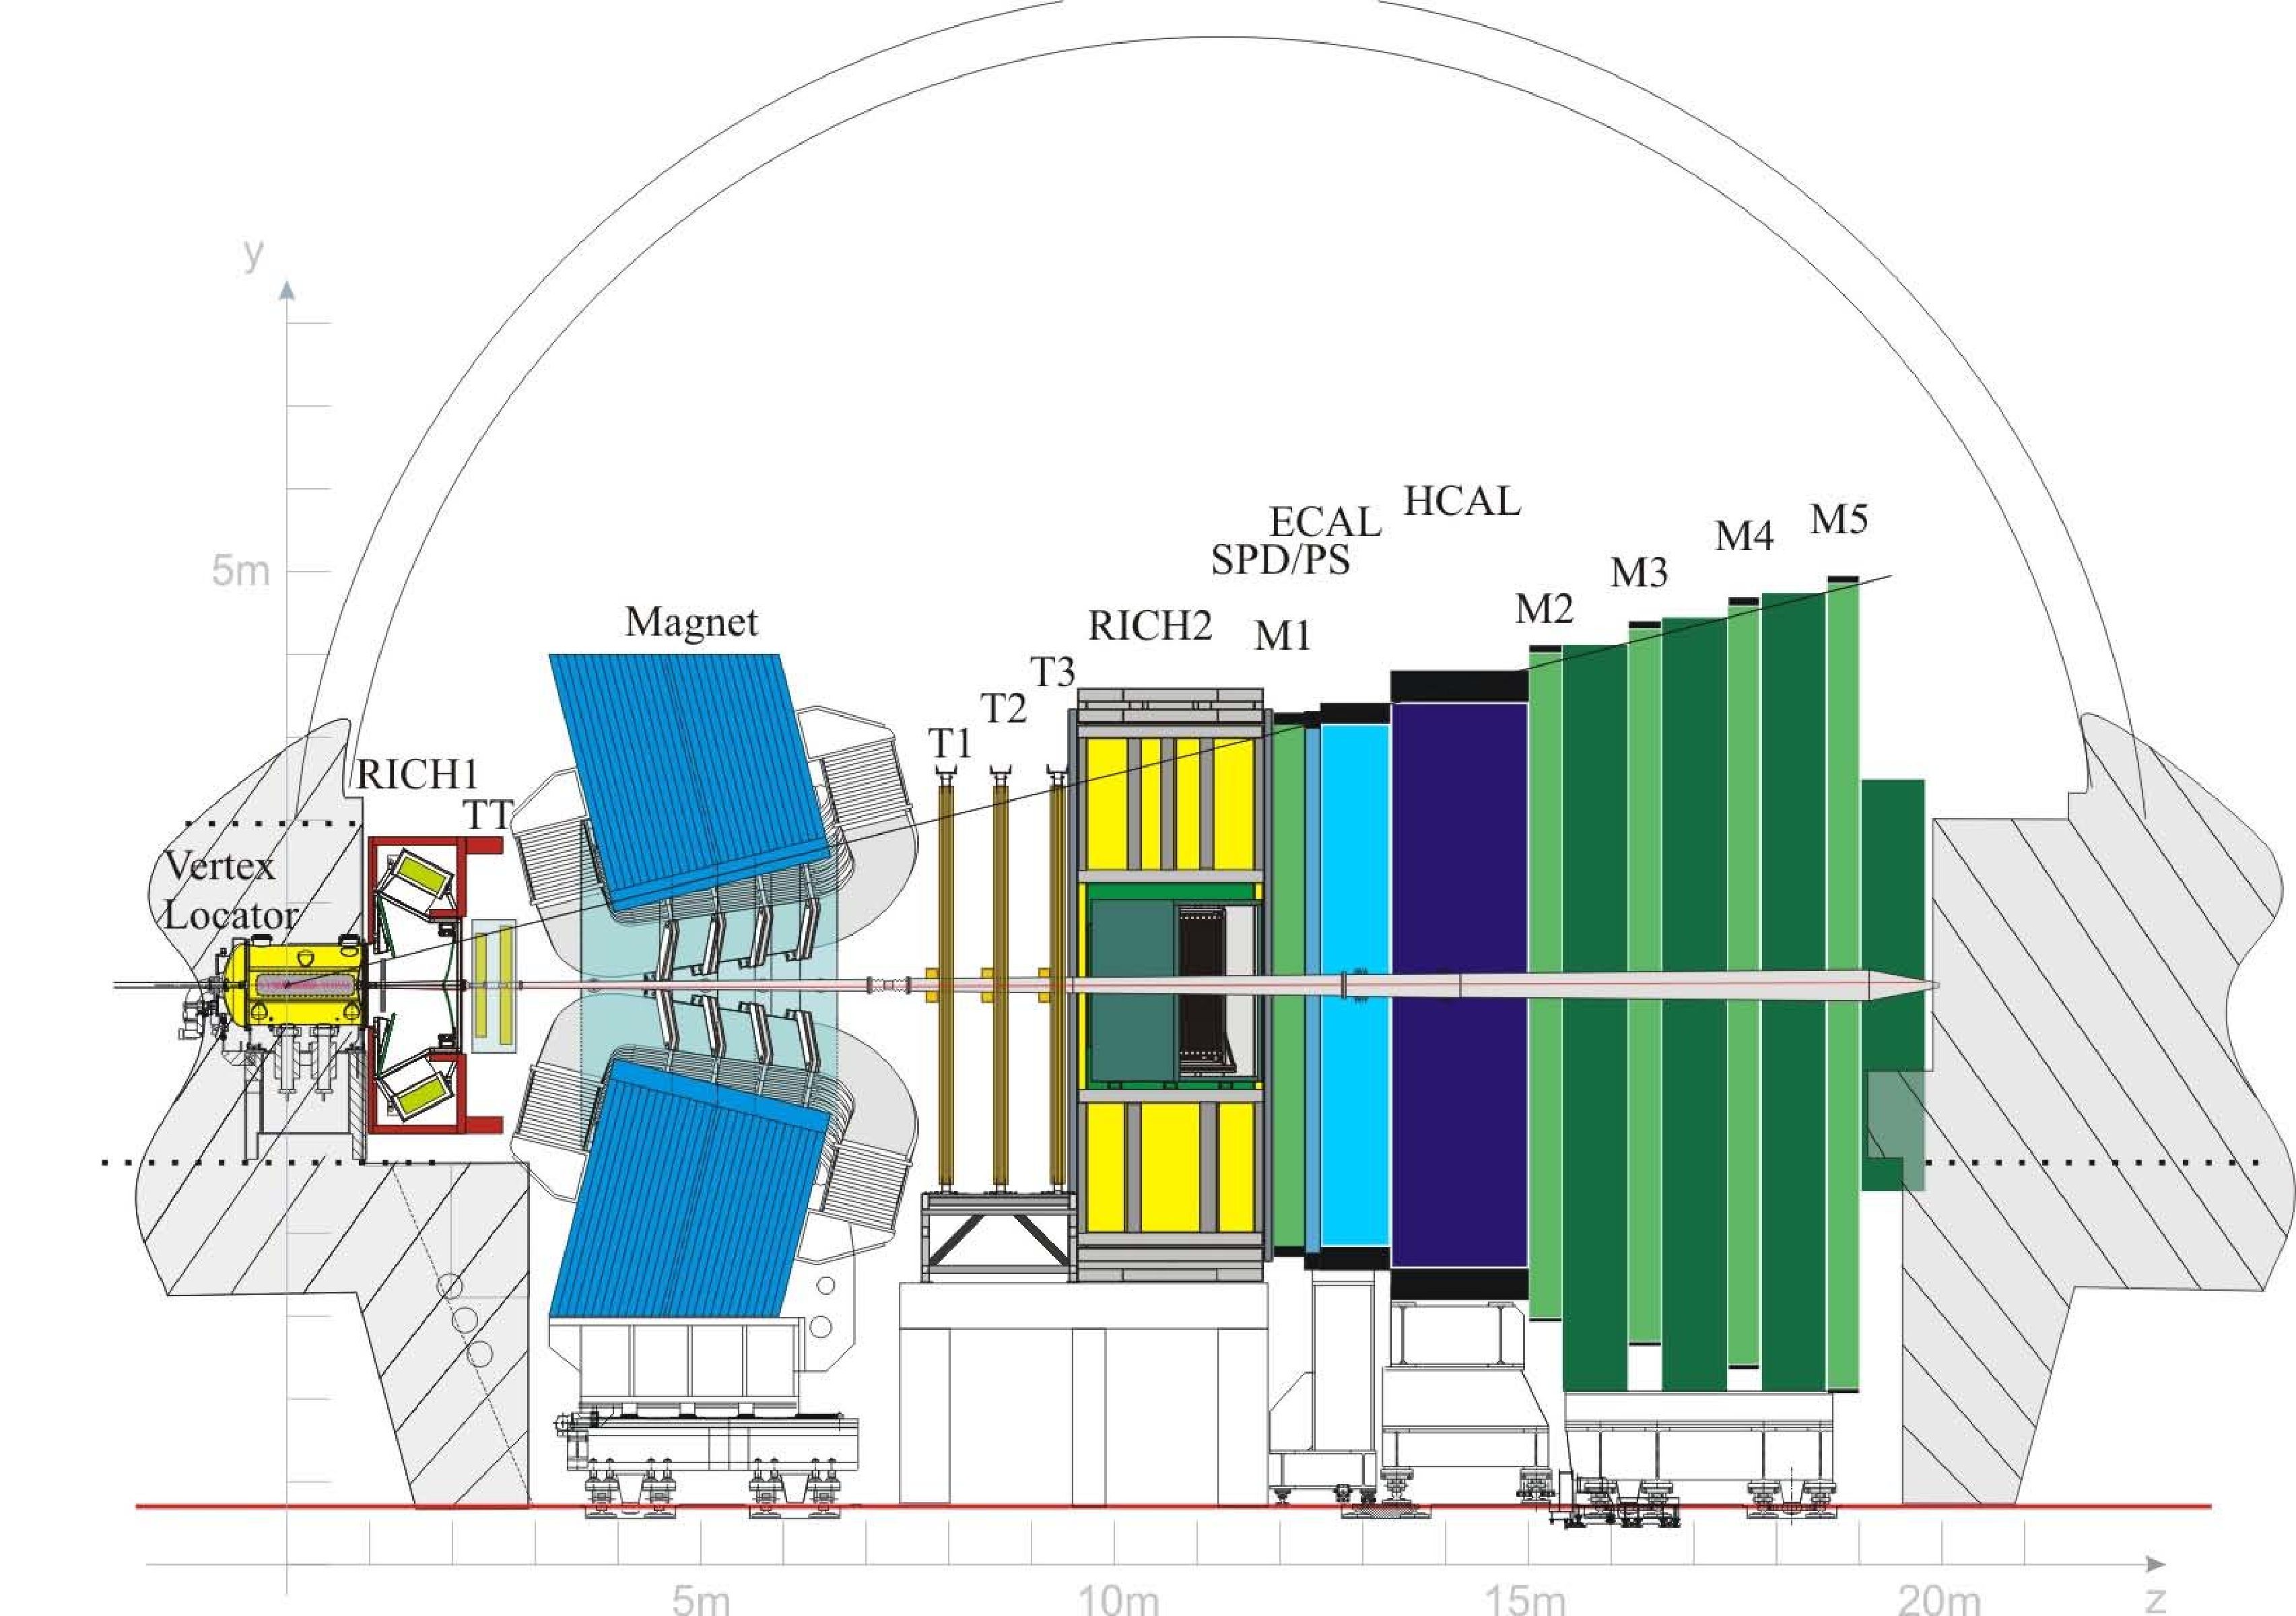
\includegraphics[width=\textwidth]{04-Detector/figs/Lhcbdetektor.pdf}
\caption{Schematic view on the \lhcb detector\cite{Alves:2008zz}.}
\label{fig:detector:scheme}
\end{figure}
Instrumenting only this part of the space has been found to be an optimal
compromise between cost and output for \lhcb's desired physics program, which
is mainly to study particles containing \bquark or \cquark quarks. Simulations
of the correlation between the angular distribution of \bbbar quark pairs (see
\cref{fig:detector:bbbar}) show that the \bquark and \bquarkbar quarks are
mainly produced in quite small cones around the beam axis. Of course, half of
the \bbbar quark pairs are going backwards but about \SI{25}{\percent} of all
\bbbar quark pairs are inside the instrumented \SI{4.5}{\percent} of the whole
space.
\begin{figure}[htb]
\centering
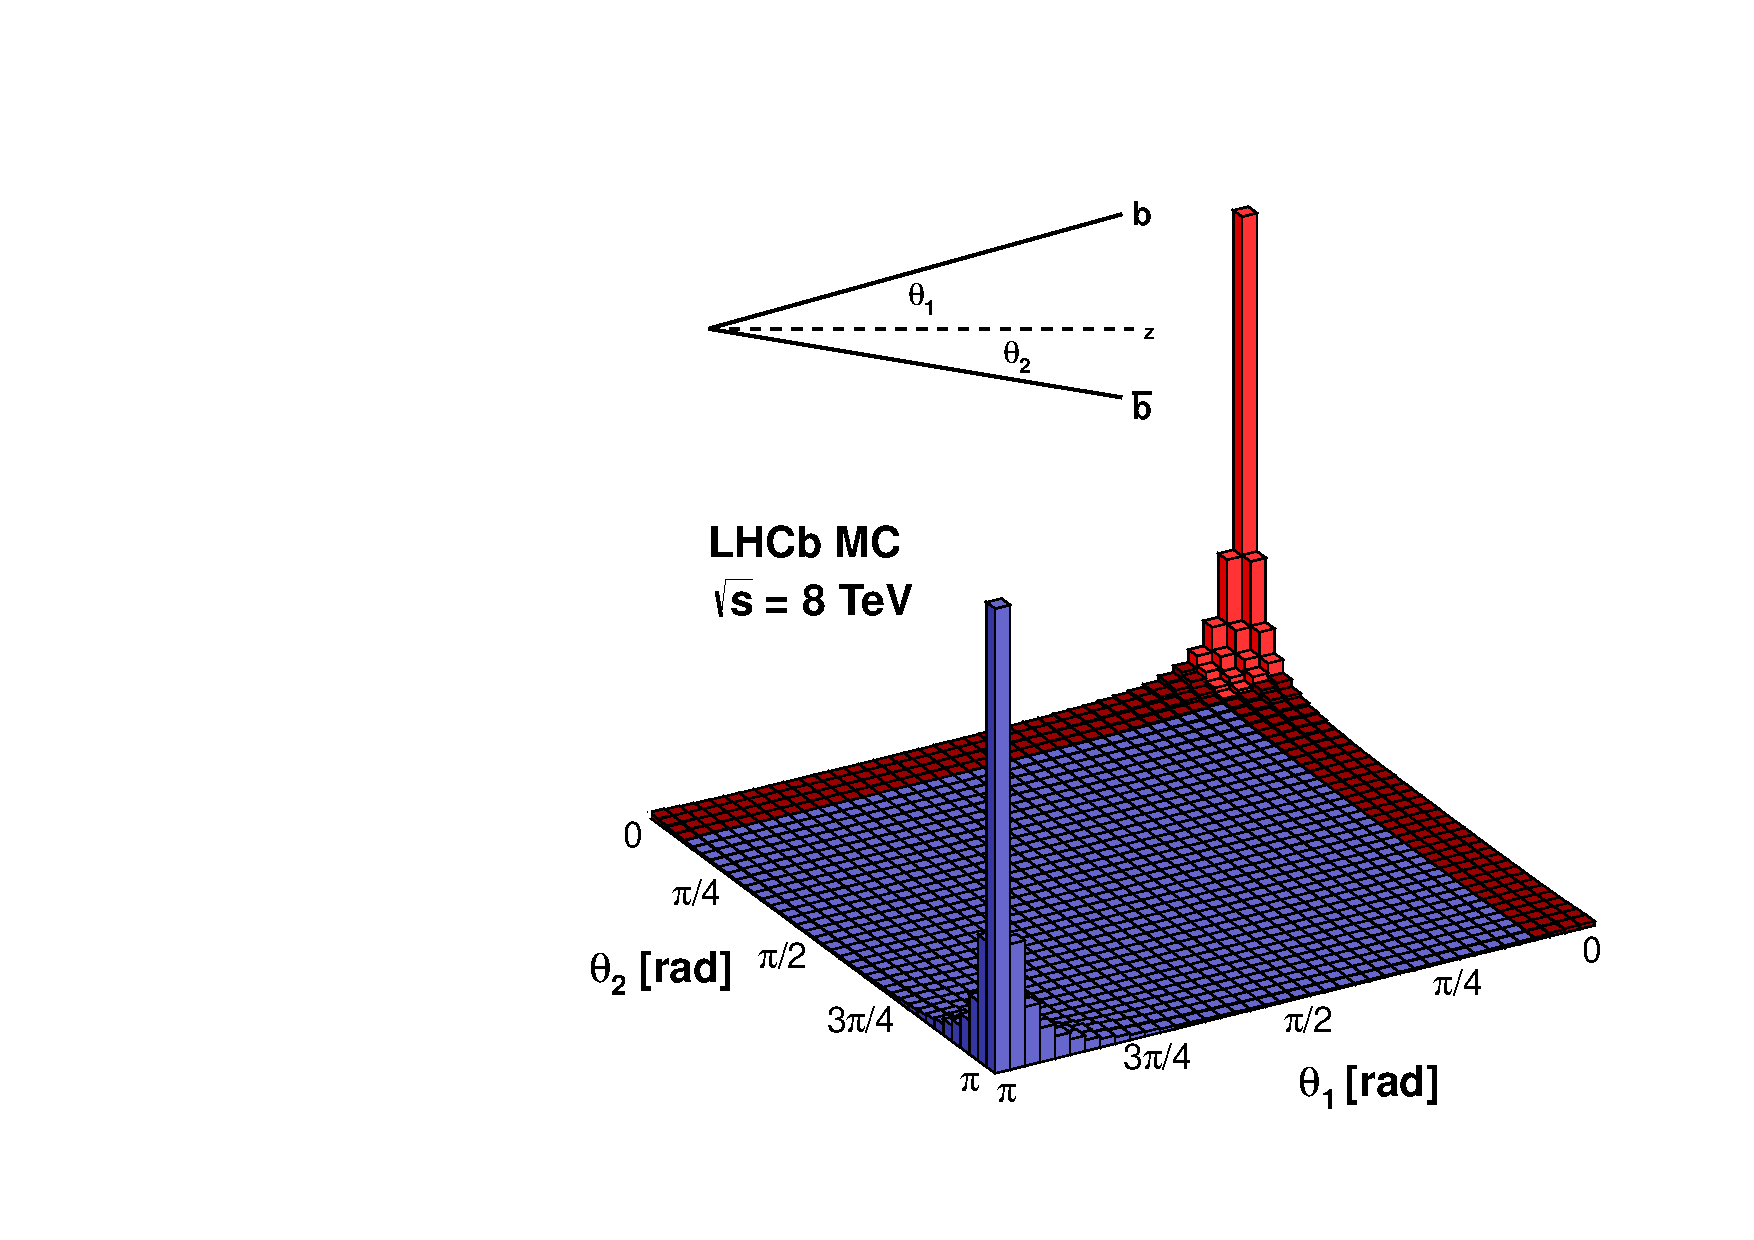
\includegraphics[width=0.49\textwidth]{04-Detector/figs/bbbarcorrelation.pdf}
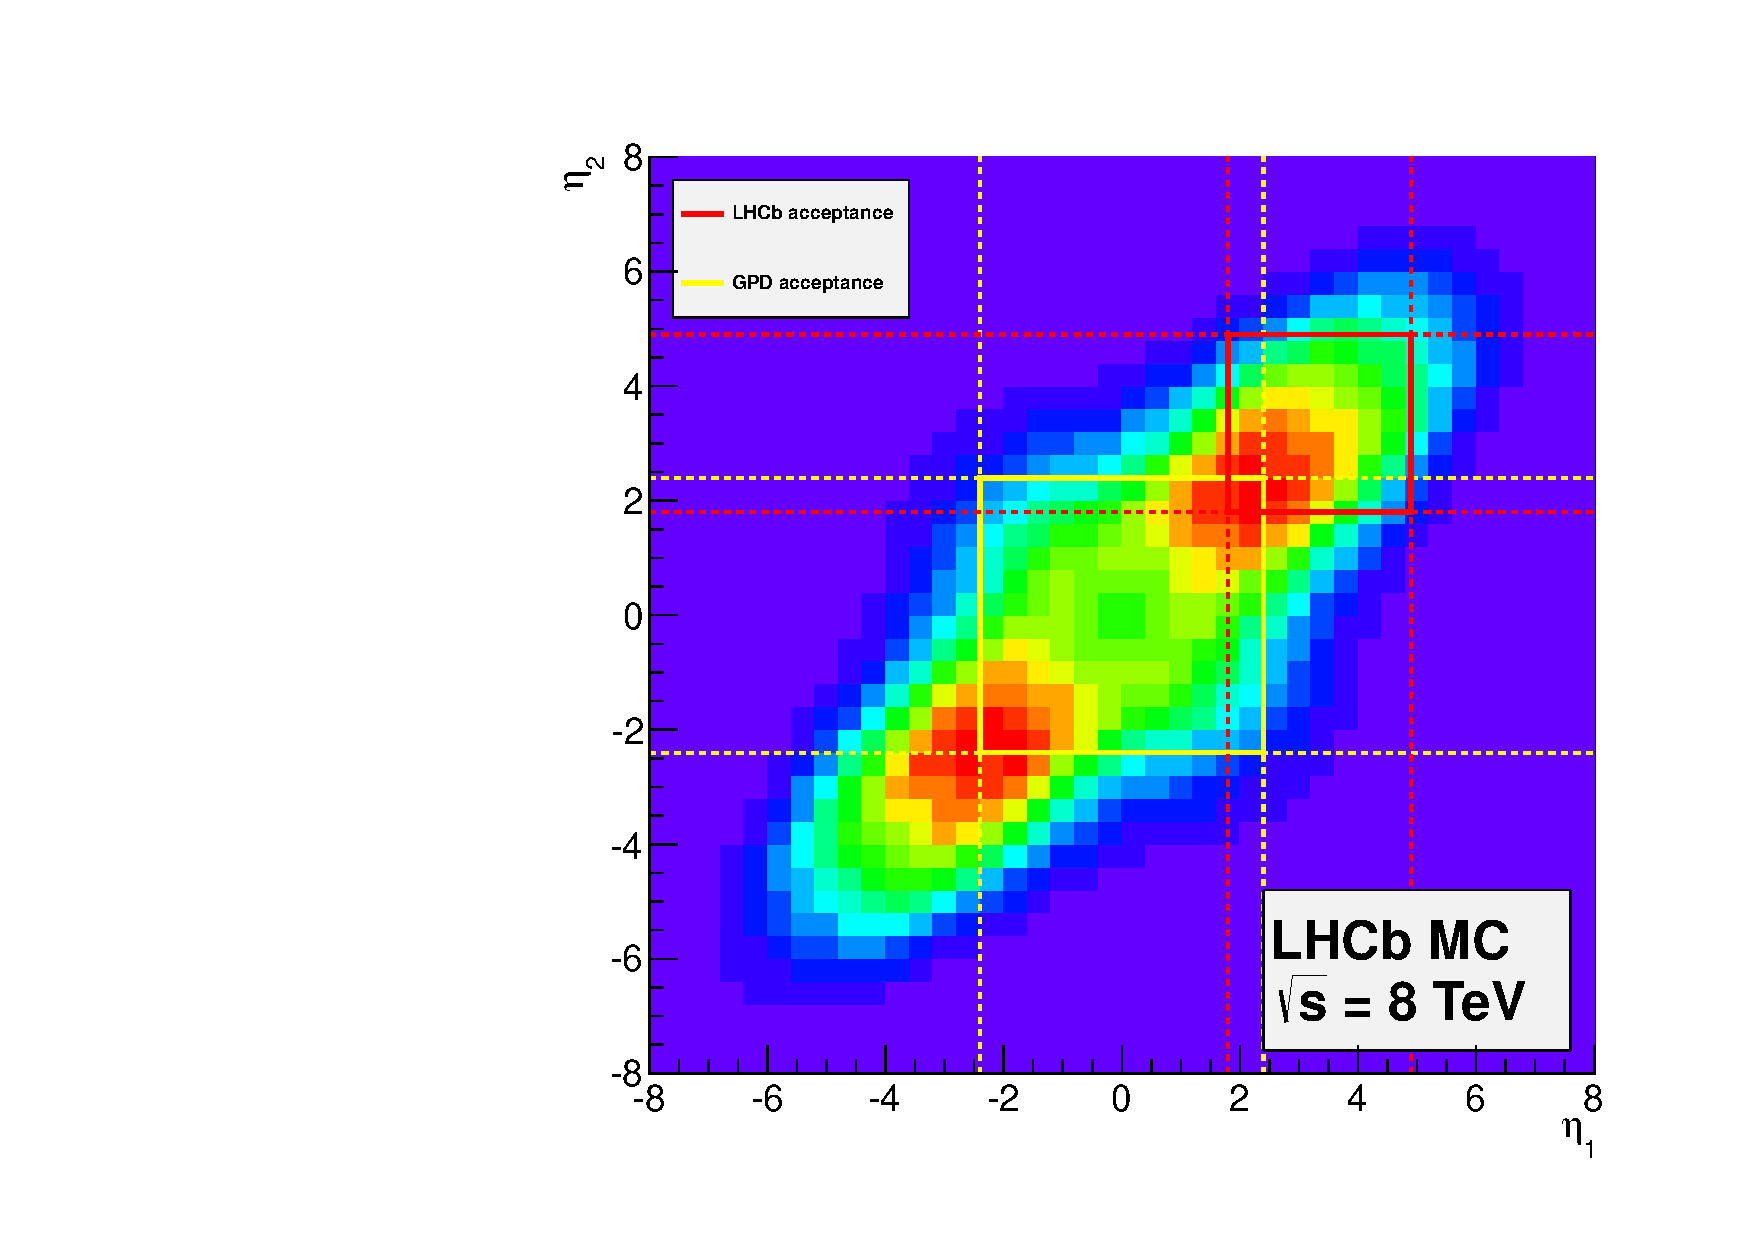
\includegraphics[width=0.49\textwidth]{04-Detector/figs/bbbaracceptance.pdf}
\caption{Correlation of angular acceptance (left) and pseudorapidity (right)
of \bbbar quark pairs. The frequency of produced \bbbar quark pairs is
indicated by the bin content in the plot showing the angular acceptance and by
the colour code in the plot of the pseudorapidities, where purple means low
and red corresponds to high. The region marked in red (left) respectively the
region in the red square is instrumented by the \lhcb detector.}
\label{fig:detector:bbbar}
\end{figure}

More details on the structure of the \lhcb detector can be found in
Ref.~\cite{Alves:2008zz} and an overview of the performance is given in
Ref.~\cite{LHCb-DP-2014-002}.

\subsection*{Vertexing and tracking}
\label{subsec:tracker}

The tracking system consists of several detector components, one of which is a
dipole magnet, which bends the tracks of charged particles with an integrated
magnetic field of \SI{4}{Tm}. To be able to study charge-dependent detection
asymmetries the polarity of the dipole magnet is reversed periodically
throughout data-taking. The momentum of the track can be derived from the
curvature radius. To determine the curvature radius, information from tracking
detector elements located upstream and downstream of the magnet is needed. The
$pp$ interaction region is surrounded by a silicon-strip vertex locator
(VELO)~\cite{LHCb-DP-2014-001}, which delivers the most precise information on
the position of the tracks and vertices due to being installed very closely
around the beam pipe. It is composed of 42 modules with R and $\phi$ sensors,
which measure the positions of the tracks in cylindrical coordinates. Each
module is a half disk (see \cref{fig:detector:velo}), which can be pulled to a
proximity of \SI{5}{\milli\metre} to the beam axis. However, this is only done
for stable beam conditions, otherwise the modules could be destroyed by the
beam. To monitor the beam position a dedicated detector component called Beam
Conditions Monitor (BCM) is installed at two locations in the vicinity of the
beam. Via eight diamond sensors, which have been proven to be very
radiation-hard, each station determines the particle flux and can trigger a
beam dump in case of instabilities, which occur especially during the
injection of proton bunches. The importance of this system is underlined by
the fact that it has its own power supply and constantly reports its status.
If no information from the BCM is received a beam dump is also initiated. The
VELO achieves a single hit resolution of up to \SI{4}{\mum} at an efficiency
of more than \SI{99}{\percent}. The disks are arranged in a way that
guarantees that even at the outermost acceptance of \SI{300}{mrad} tracks hit
at least three VELO stations (see \cref{fig:detector:velo}).
\begin{figure}[htb]
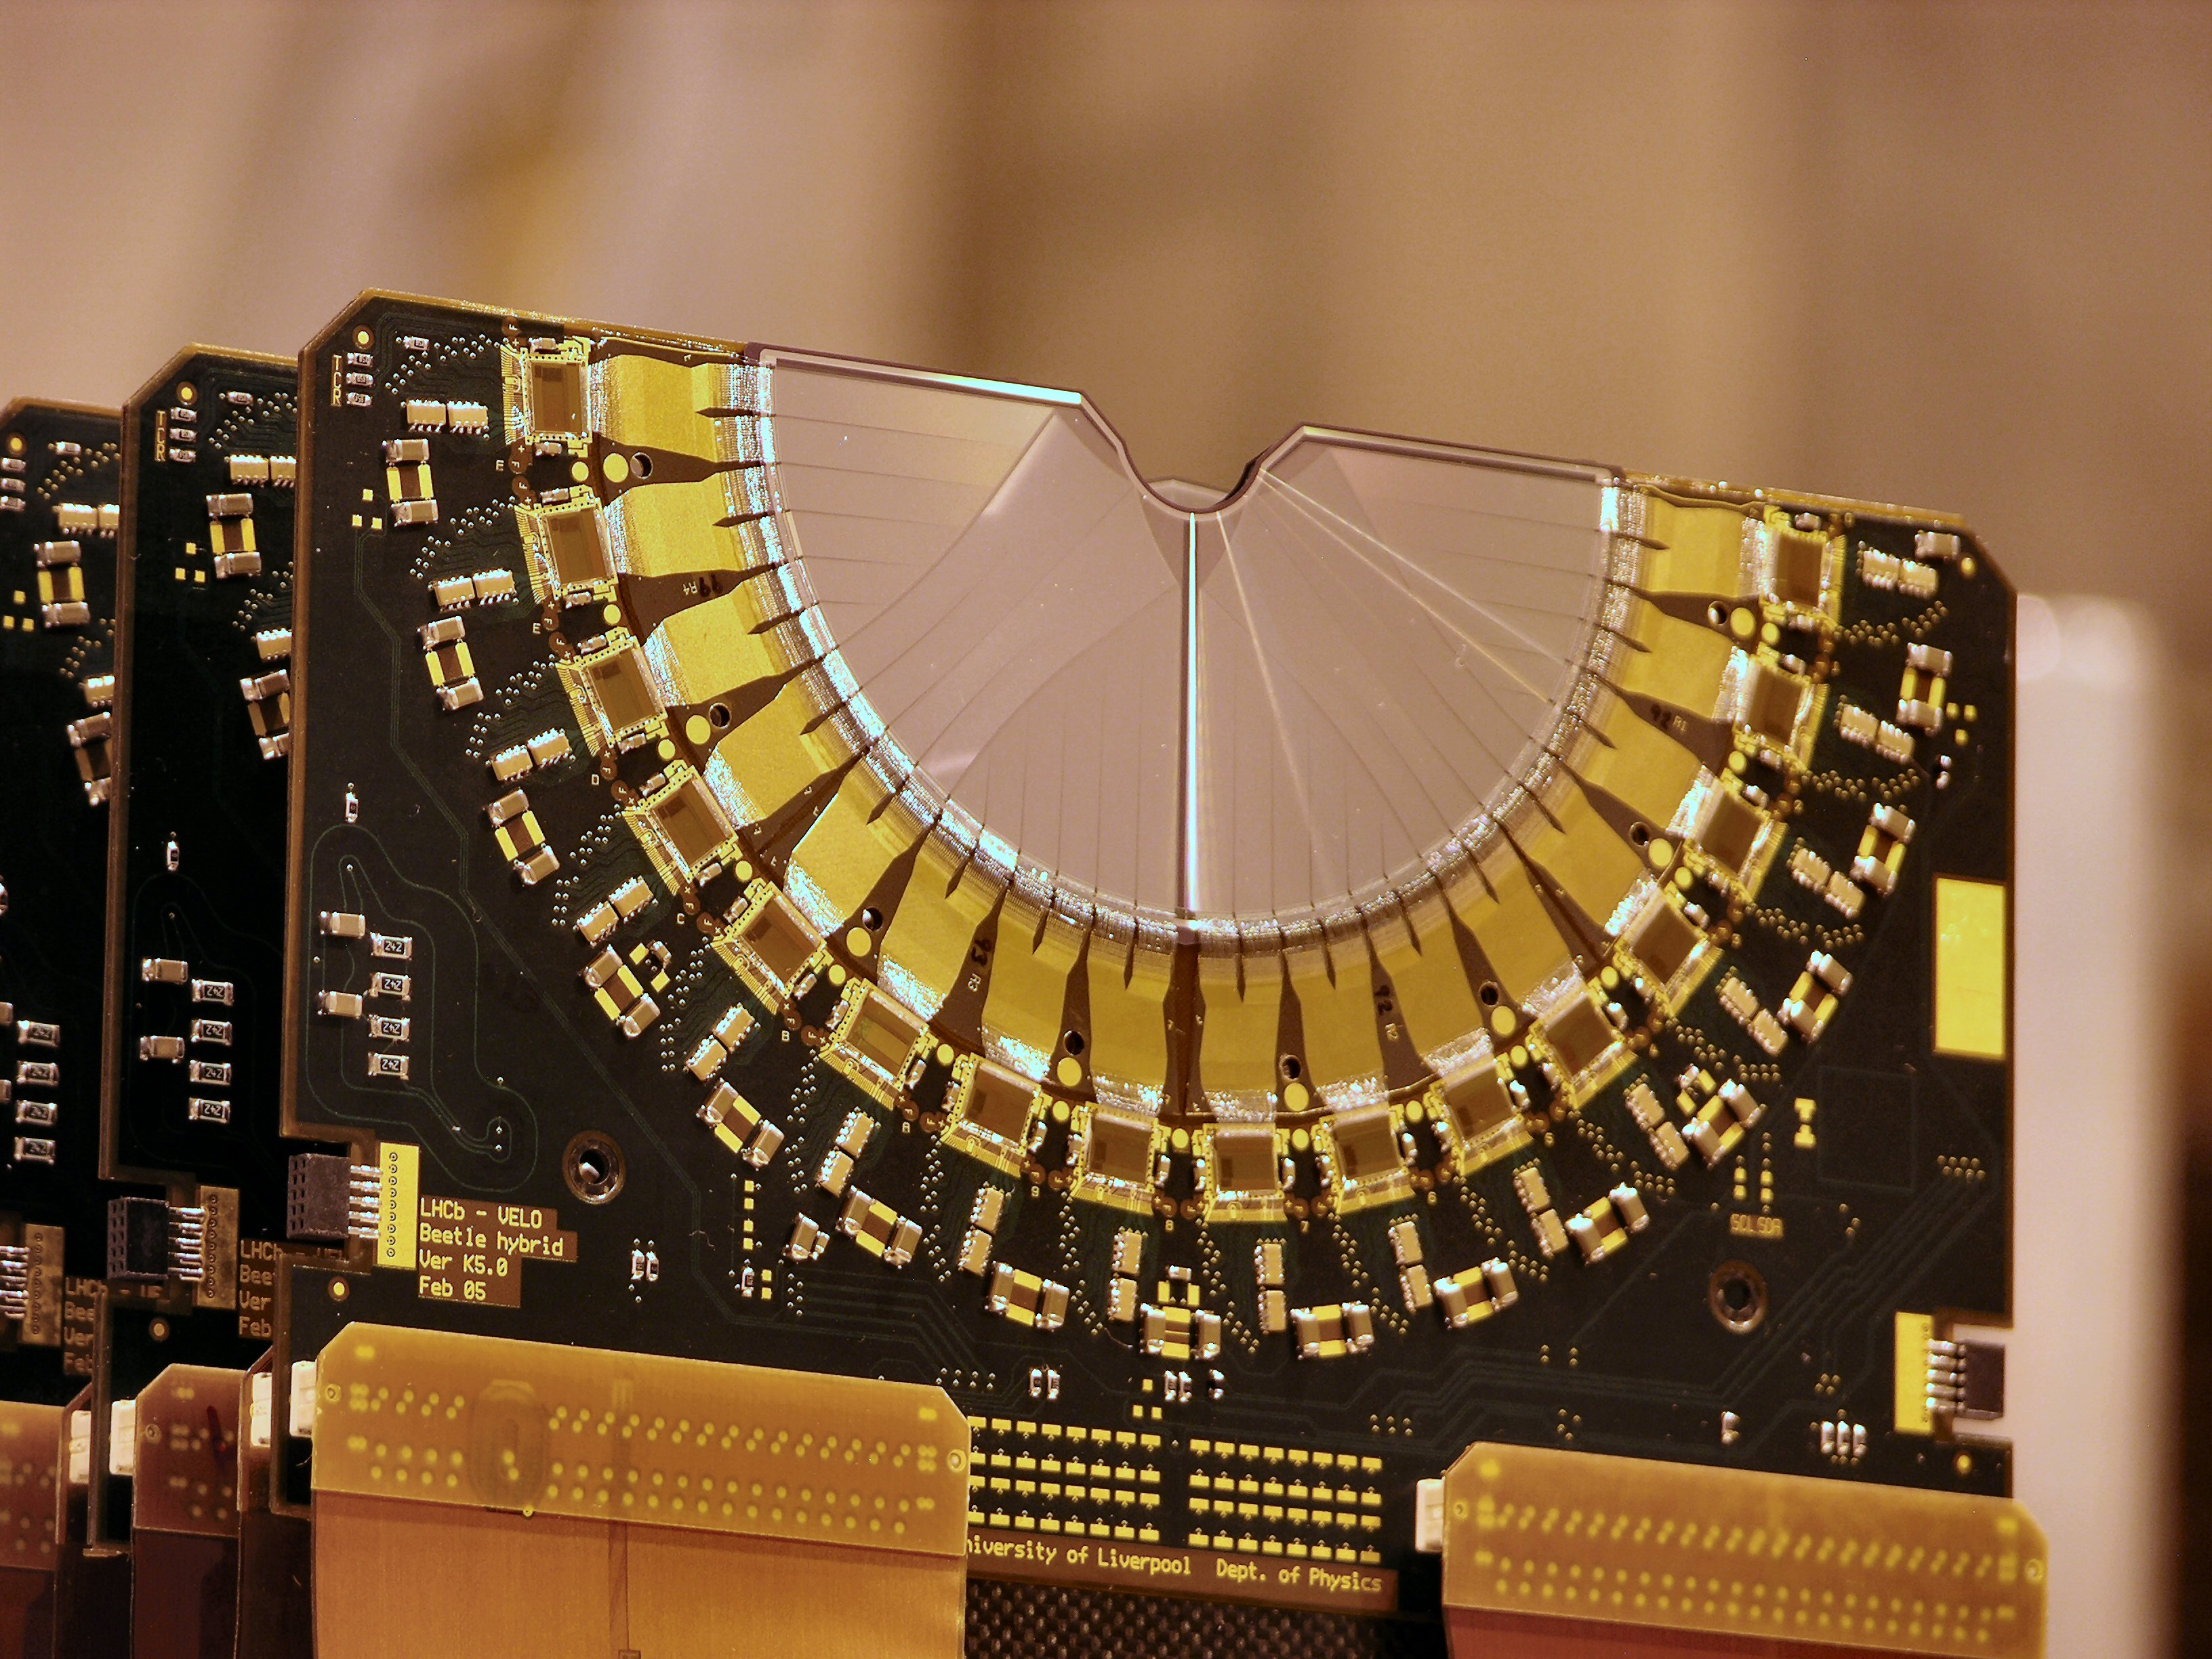
\includegraphics[width=0.4\textwidth]{04-Detector/figs/VELO.jpg}
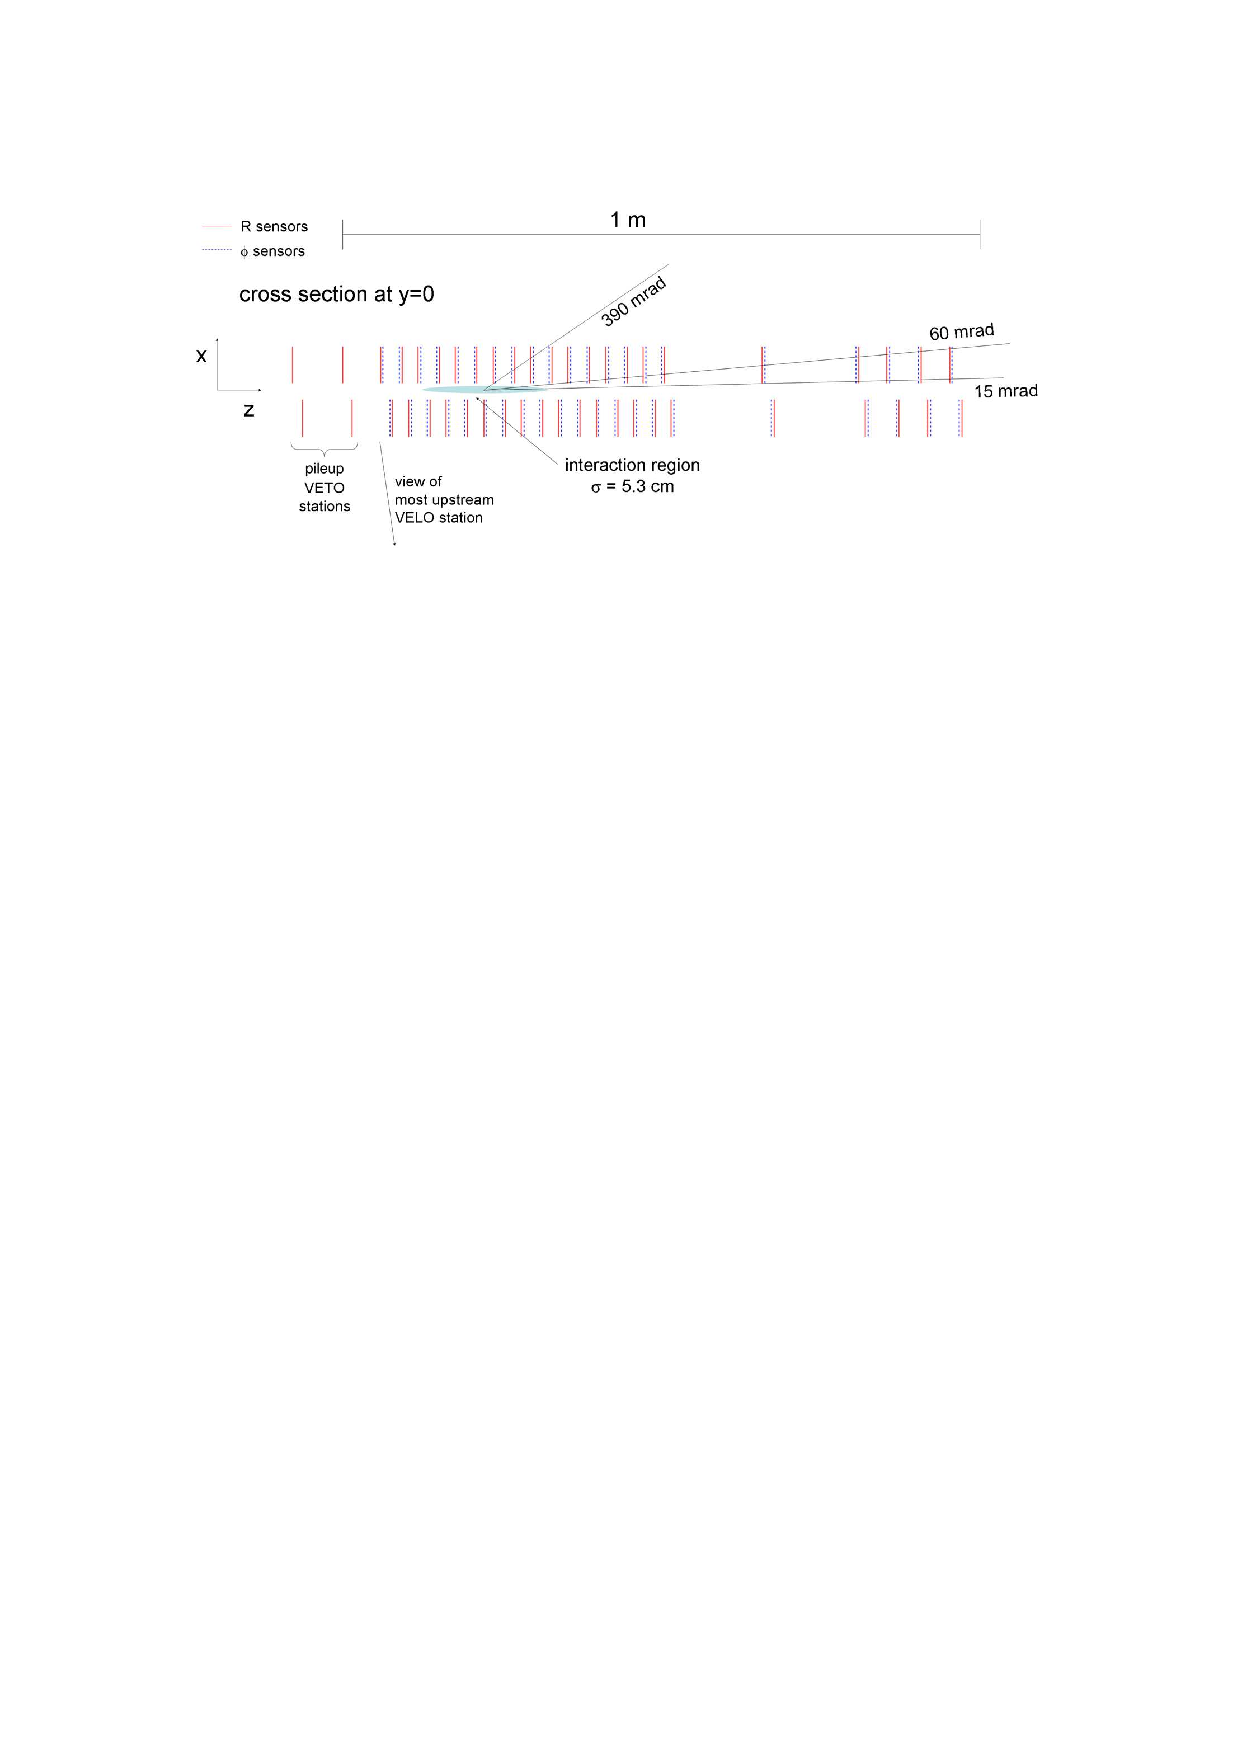
\includegraphics[width=0.59\textwidth]{04-Detector/figs/AnordnungVELOStationen.pdf}
\caption{View on a single VELO half disk (left) and arrangement of all VELO
modules~\cite{Alves:2008zz}.}
\label{fig:detector:velo}
\end{figure}
One of the main purposes of the VELO is to precisely determine the position of
the proton-proton interaction called primary vertex (PV) and the displaced
secondary decay vertices of long-lived particles like \Bd mesons. The impact
parameter (IP), which is the minimum distance of a track to a PV, is measured
depending on the transversal momentum \pT with a spatial resolution of
$(15+29/\pt)\mum$ (\pT given in units of \si{\gevc}).

Between VELO and dipole magnet there is another silicon-strip detector, the
tracker turicensis (TT). Like the three tracking stations located downstream
of the magnet, which are subdivided into an inner silicon-strip tracker and an
outer straw drift tube detector~\cite{LHCb-DP-2013-003}, it is built of four
layers. While the first and last layer are arranged vertically, the inner
layers are tilted by \SI{-5}{\degrees} and \SI{+5}{\degrees}, respectively.
Charged particles create electron-hole pairs in the silicon-strip detectors
inducing a measurable current. A hit efficiency of at least
\SI{99.7}{\percent} and a hit resolution of \SI{55}{\mum} and better is
achieved during data-taking in 2011 and 2012~\cite{LHCb-DP-2014-002}. The
straw drift tubes of the outer tracker are filled with a gas mixture of
\SI{70}{\percent} Ar, \SI{28.5}{\percent} CO$_2$ and \SI{1.5}{\percent} O$_2$.
The addition of the oxygen reduces the ageing rate~\cite{Bachmann:2010zz}.
Passing particles ionise the gas. Timing measurements on how long it takes for
the electrons to reach the anode in the middle of the tube allow to
reconstruct the position of the hit. In total, the tracking system provides a
relative precision on the measurement of the momentum that varies from
\SI{0.5}{\percent} at low momentum to \SI{0.8}{\percent} at
\SI{100}{\gevc}~\cite{LHCb-DP-2014-002}.

Different track types are distinguished based on which detector components
provide information on the trajectory of the track. The category with the best
mass, momentum and vertex resolution is the long category. Long tracks
originate in the vertex detector and leave hits in all subsequent tracking
stations. Long-lived particles like \KS mesons might decay outside the VELO.
If their tracks are detected in the TT and, after passing the magnet, in the
tracking stations they are referred to as downstream. These two track
categories are the only ones used in the analyses described in this thesis.
Furthermore, tracks are classified as VELO tracks, if they have only left hits
in the VELO, as upstream tracks, if in addition the TT delivers information,
or as T tracks, if they are solely reconstructed in the tracking stations
downstream the magnet.


\subsection*{Particle identification}
\label{subsec:teilchenidentifizierung}

Apart from detecting the tracks and reconstructing their trajectory it is
important to estimate the identity of the particles. To distinguish pions from
kaons and protons two ring-imaging Cherenkov (RICH)
detectors~\cite{LHCb-DP-2012-003} are used, which are installed between VELO
and TT respectively downstream of the tracking stations. The RICH detector
upstream of the magnet is filled with $\mathrm{C_4F_{10}}$ and during Run I
additionally with Aerogel. It is designed for particles with momenta in the
range of \SIrange{1}{60}{\gevc}. Higher momentum particles are detected by the
second RICH detector, which is filled with $\mathrm{CF_4}$. When particles
pass through these materials with a speed greater than the speed of light in
the medium photons are emitted. The light is guided to hybrid photo detectors
by a system of mirrors (see \cref{fig:detector:rich}). From the radius of the
light cones and the measurement of the momentum a particle hypothesis can be
constructed.
\begin{figure}[htb]
\centering
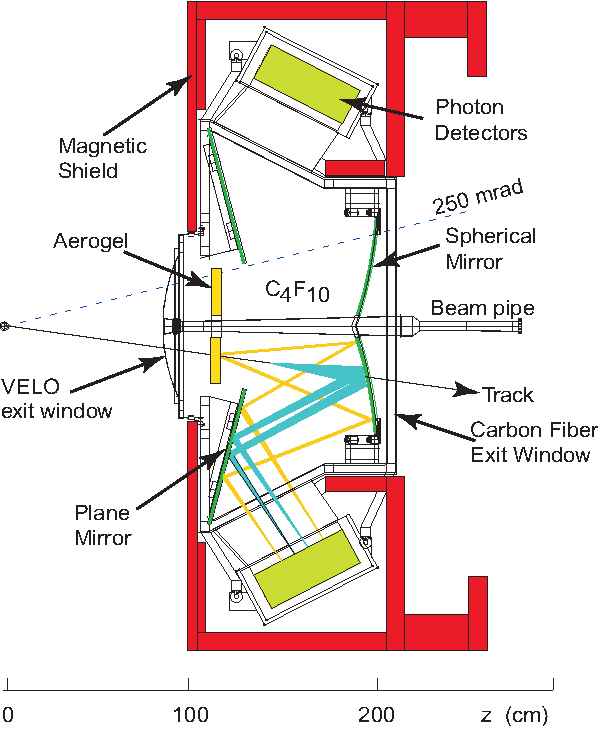
\includegraphics[width=0.25\textwidth]{04-Detector/figs/rich1-2d.pdf}
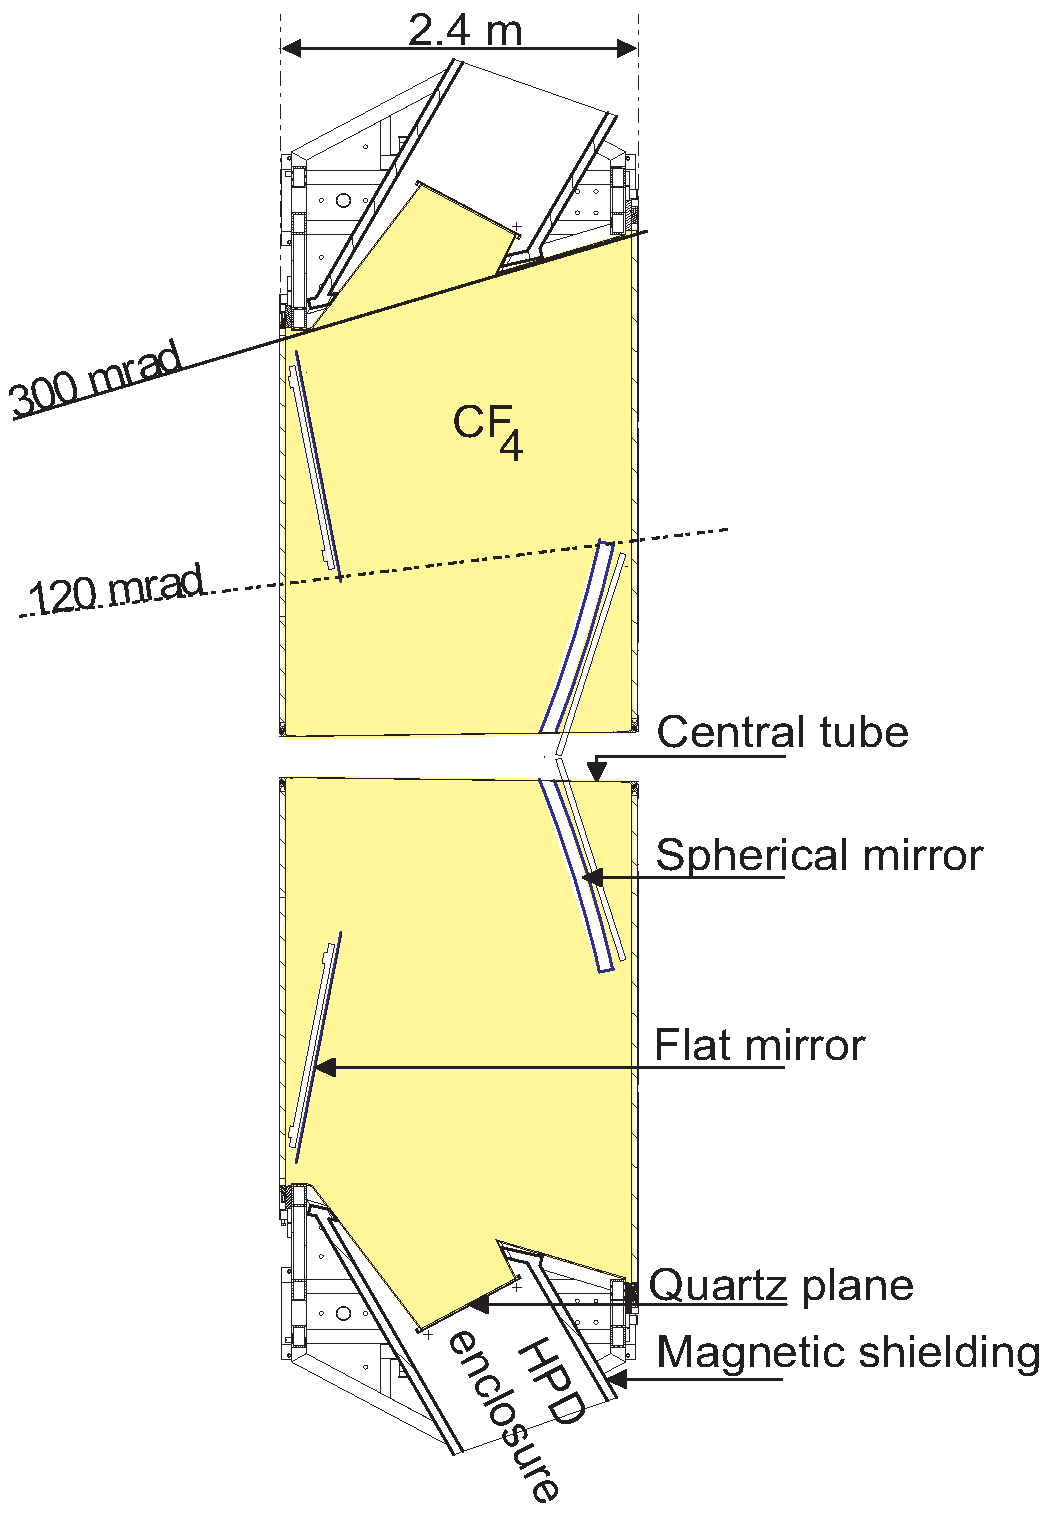
\includegraphics[width=0.25\textwidth]{04-Detector/figs/rich2_schematic.pdf}
\caption{Side view schematic layout of RICH 1 (left) and top view schematic of
RICH 2 (right)~\cite{Alves:2008zz}.}
\label{fig:detector:rich}
\end{figure}
While photons and electrons are identified by an electromagnetic calorimeter
(ECAL), the energy of protons, neutrons and other long-lived hadrons is
measured in a hadronic calorimeter (HCAL). To suppress background from charged
and neutral pions there is a preshower (PS) respectively a Scintillator Pad
Detector (SPD) in front of the ECAL. The thickness of the lead in the PS is
chosen as a compromise between energy resolution and trigger
performance~\cite{Preshower}. The calorimeters are built of alternating layers
of metal and plastic. Polystyrene molecules in the plastic are excited by
particle showers produced in the metal plates and produce ultraviolet light,
whose amount is proportional to the energy of the incident particle. The least
interacting charged particles are muons, which are identified by five stations
of multi-wire proportional chambers (MWPC) filled by a gas mixture of $\mathrm{Ar,
CO_2}$ and $\mathrm{CF_4}$. Four of them are right at the end of the detector
downstream of the calorimeters and one is located in between the second RICH
and the calorimeter system. To stop the muons \SI{80}{cm} thick layers of iron
are put between the last four muon stations. Only muons with a momentum $p >
\SI{6}{\gevc}$ pass the whole detector. The detection of the muons is based on
ionisation of the gas in the MWPCs. An electric field accelerates the ions and
electrons. The emerging current is proportional to the energy of the muon.


%!TEX root = ../main.tex

\section{The LHCb trigger system}
\label{sec:detector:trigger}

Deliberately, the instantaneous luminosity at \lhcb is reduced to
$\SI{4e32}{\cm^{-2}s^{-1}}$, which is significantly lower than at the other
three experiments at the \lhc. Though, the partial beam loss with time can be
compensated by adjusting of the beam crossing so that a constant luminosity
level can be kept throughout the whole fill. Nevertheless, it is not possible
to store the data of all visible proton-proton collisions. Instead, a two
stage trigger system consisting of a hardware (L0) and a subsequent software
level (HLT) is deployed. At the hardware trigger stage, which runs
synchronously with the bunch crossing rate of \SI{40}{\mega\hertz}, events are
required to contain at least one muon with a high \pt (\texttt{L0Muon}), or
two muons with a minimal product of their \pT (\texttt{L0DiMuon}), or a hadron
(\texttt{L0Hadron}), a photon (\texttt{L0Photon}) or an electron
(\texttt{L0Electron}), which deposit high transverse energy in the
calorimeters. Additionally, the number of allowed hits in the SPD is limited.
These requirements reduce the data rate to \SI{1}{\mega\hertz}, at which the
full detector can be read out. The L0 signal efficiency varies a lot between
muons and hadrons. While dimuon final states are triggered with more than
\SI{90}{\percent} efficiency, for fully hadronic final states like $\Dp\Dm$
only around \SI{60}{\percent} are reached. The high level trigger (HLT) is a
\cpp application, which runs on an event filter farm of several thousand CPU
nodes. It is again split into two stages. In the HLT1 basically the decisions
of the L0 are checked. Due to the reduced data rate some more time is
available. For all events the VELO tracks are reconstructed and a partial
event reconstruction of all charged particles with $\pt > \SI{500}{\mevc}$ in
2011 and $\pt > \SI{300}{\mevc}$ in 2012 is performed. This improves the
momentum resolution and enables to calculate some invariant masses. The
\texttt{Hlt1TrackMuon} trigger line requires a high \pt muon with a \chisqip
with respect to any primary interaction greater than 16, where \chisqip is
defined as the difference in \chisq of a given PV reconstructed with and
without the considered track. %which is incompatible with originating from any PV in the event. 
The \texttt{Hlt1DiMuonHighMass} trigger line accepts events if they contain
two muons that form a good common vertex with an invariant mass above
\SI{2.7}{\gevcc}. In HLT2, a full reconstruction of the event is performed.
Therefore, it is possible to further tighten the requirements applied in HLT1.
Furthermore, for the \texttt{Hlt2DiMuonDetachedJPsi} trigger line a
requirement on the flight distance is imposed. For hadrons, it is typically
searched for two-, three- or four-track secondary vertices, which are
identified via a multivariate algorithm~\cite{BBDT}.

The total output rate after all trigger stages has been increased from
\SI{3.5}{\kilo\hertz} in 2011 to \SI{5}{\kilo\hertz} in 2012 and
\SI{12.5}{\kilo\hertz} in Run II.

In the offline selection, trigger signals are associated with reconstructed
particles. Selection requirements can therefore be made on the trigger
selection itself and on whether the decision was due to the signal candidate
(TOS), other particles produced in the $pp$ collision (TIS), or a combination
of both.


%!TEX root = ../main.tex

\section{The LHCb software (1 page)}
\label{sec:detector:software}

\subsection{Reconstruction (1 page)}
\label{sec:detector:software:reconstruction}

\subsection{Stripping (1 page)}
\label{sec:detector:software:stripping}

\subsection{Monte Carlo simulation (1 page)}
\label{sec:detector:software:simulation}